

\title{Helicorder Class for GISMO}                                                  
\author{Dane Ketner \\daneketner@gmail.com}
\date{\today}

\documentclass[11pt]{article}

\evensidemargin=2.0in
\oddsidemargin=-0.25in
\textwidth=7.0in
\topmargin=.2in
\headsep=0in
\headheight=-.25in
\headsep=0in
\textheight=9.7in

\usepackage{graphicx} 
\usepackage{setspace}
\usepackage{amsmath}
\usepackage{esint}
\usepackage{mcode}

\renewcommand{\topfraction}{0.85}
\renewcommand{\textfraction}{0.1}
\renewcommand{\floatpagefraction}{0.85}

\newenvironment{my_enumerate}{
\begin{enumerate}
  \setlength{\itemsep}{1pt}
  \setlength{\parskip}{0pt}
  \setlength{\parsep}{0pt}}{\end{enumerate}
}


\begin{document}

\maketitle

\clearpage


\section{Helicorder Class}

A helicorder (or seismogram) is a multi-line display of ground motion traditionally recorded onto paper around a rotating drum. The MatLAB helicorder class is designed to generate such a multi-line display and includes a number of customizeable properties that can be defined by the user, or ignored. One can think of a helicorder object \mcode{h} as a blueprint for the construction of a helicorder figure. The \mcode{build} function is then used to create the helicorder figure based on the properties in \mcode{h}. User-defined properties can override default properties if included in a call to the heliorder constructor, though all that is needed for a basic helicorder is a single waveform object input argument. In the following example, \mcode{w} is a waveform object containing three hours of data from REF:EHZ starting from March 29, 2009 starting at 07:00 UTC. Figure~\ref{hel_single_1} displays the output of the \mcode{build} function, with \mcode{fh} being the handle of the figure generated.   

\begin{lstlisting}
h = helicorder(w);
fh = build(h);
\end{lstlisting}

We see that the resulting helicorder figure contains 10 minutes of data per line, and that waveform data is printed in black. Also notice the amplitude scaling that occurs in the plot. This scaling sets the max datapoint value at the center of the trace two traces above (or below) the current trace. The max value in this plot appears to be the first earthquake on line 6 (Line 07:50:00) which reaches up to the center of line 4 (Line 07:30:00). Minutes per line, trace color, and scale are all properties that can be manually set. A user-defined property can be set upon initial creation of \mcode{h} in the following way: \mcode{h = helicorder(w, 'mpl', 15);}. This call to the constructor would override the default value of 10 with 15 minutes per line. Property values can also be set after \mcode{h} is constructed using the \mcode{set} function as follows: \mcode{h = set(h, 'mpl', 15);}.

\begin{figure}[ht] 
\centerline{\scalebox{.4} {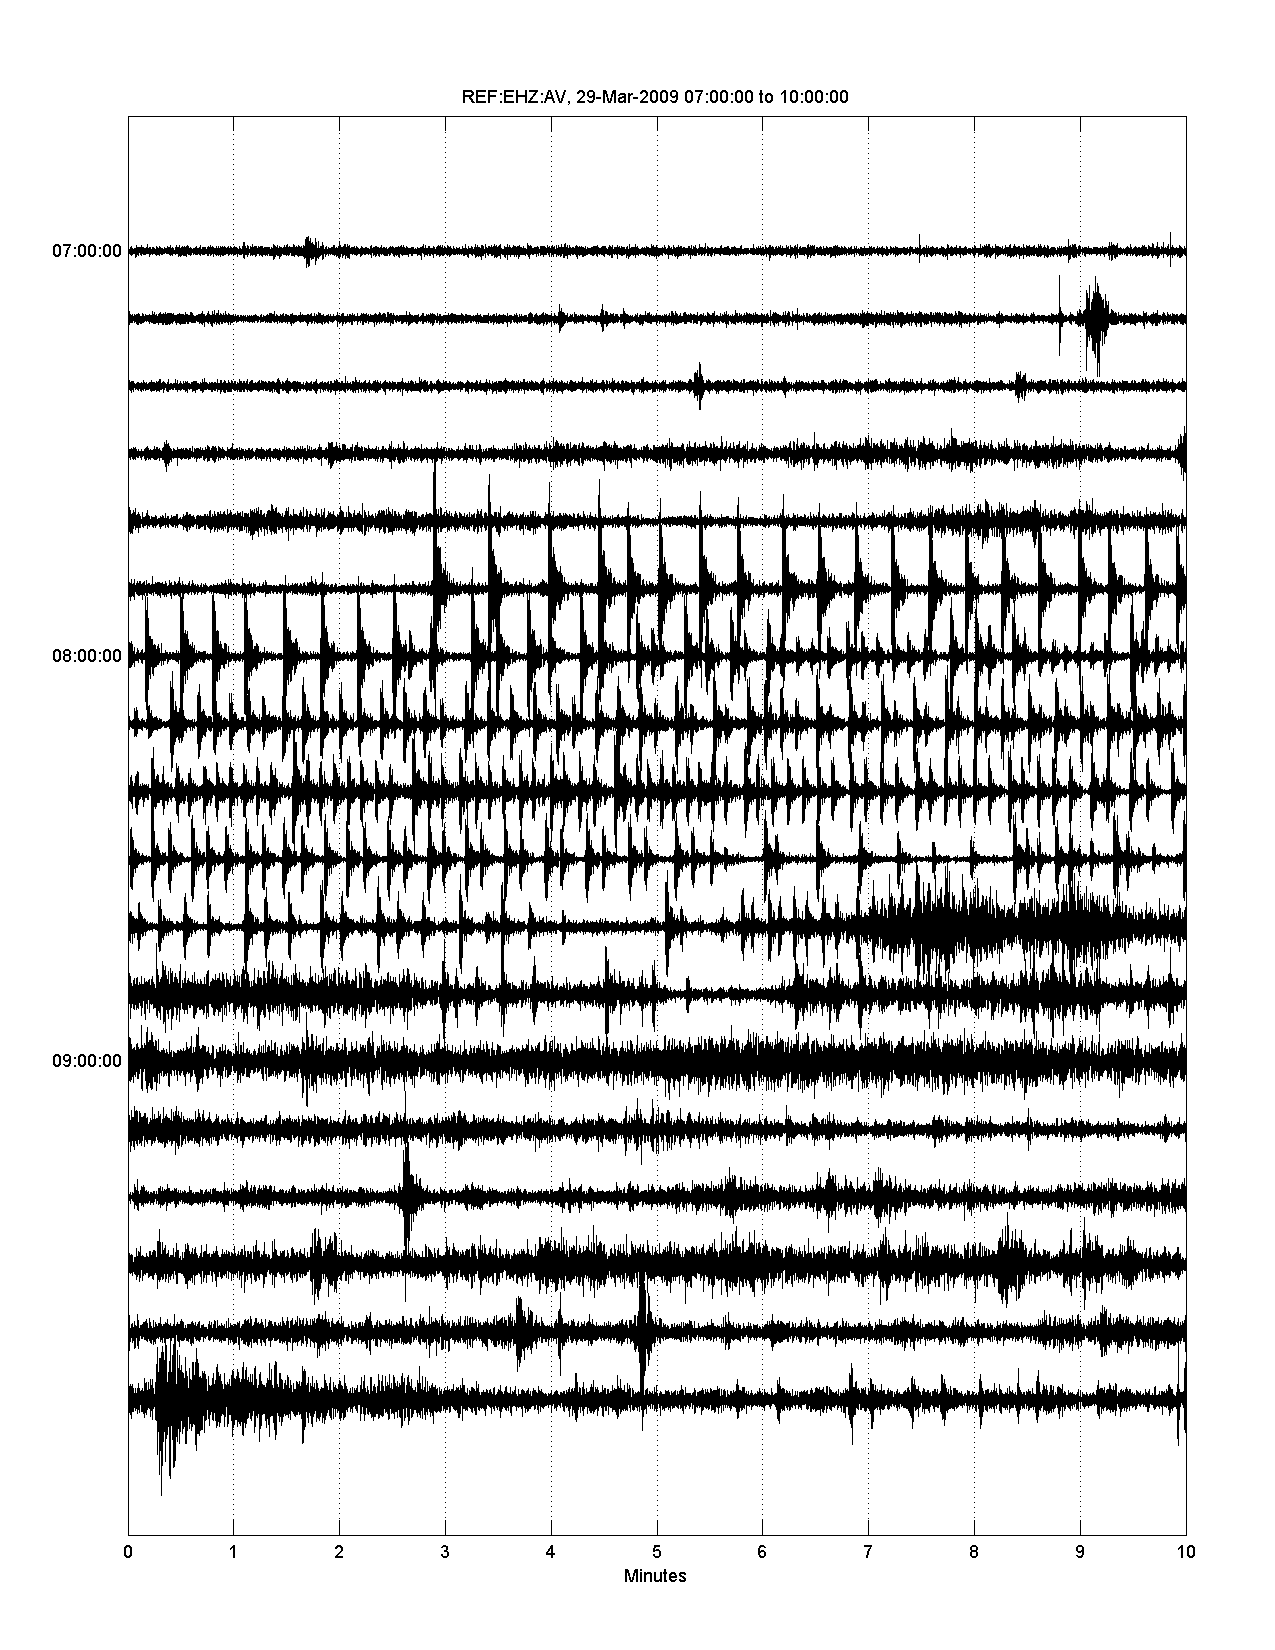
\includegraphics{hel_single_1.png}}} 
\caption{Default helicorder display for a single waveform} 
\label{hel_single_1}
\end{figure}
\clearpage

\subsection{Helicorder Multi-waveform display}

Next, let's test the default display created from an input \mcode{w} which contains multiple waveforms. In this case \mcode{w} is a 1x3 waveform object containing all three components from station REF for the same time span as the previous case. We know there will be more data to display than the previous example, so we set 20 minutes per line: \mcode{build(helicorder(w,'mpl',20))}. EHZ data is displayed in blue, EHE in black, and EHN in green in Figure~\ref{hel_alternate_1}. This multi-waveform display type is called 'alternate' which can be changed by the user in addition to the color scheme.

\begin{figure}[ht] 
\centerline{\scalebox{.6} {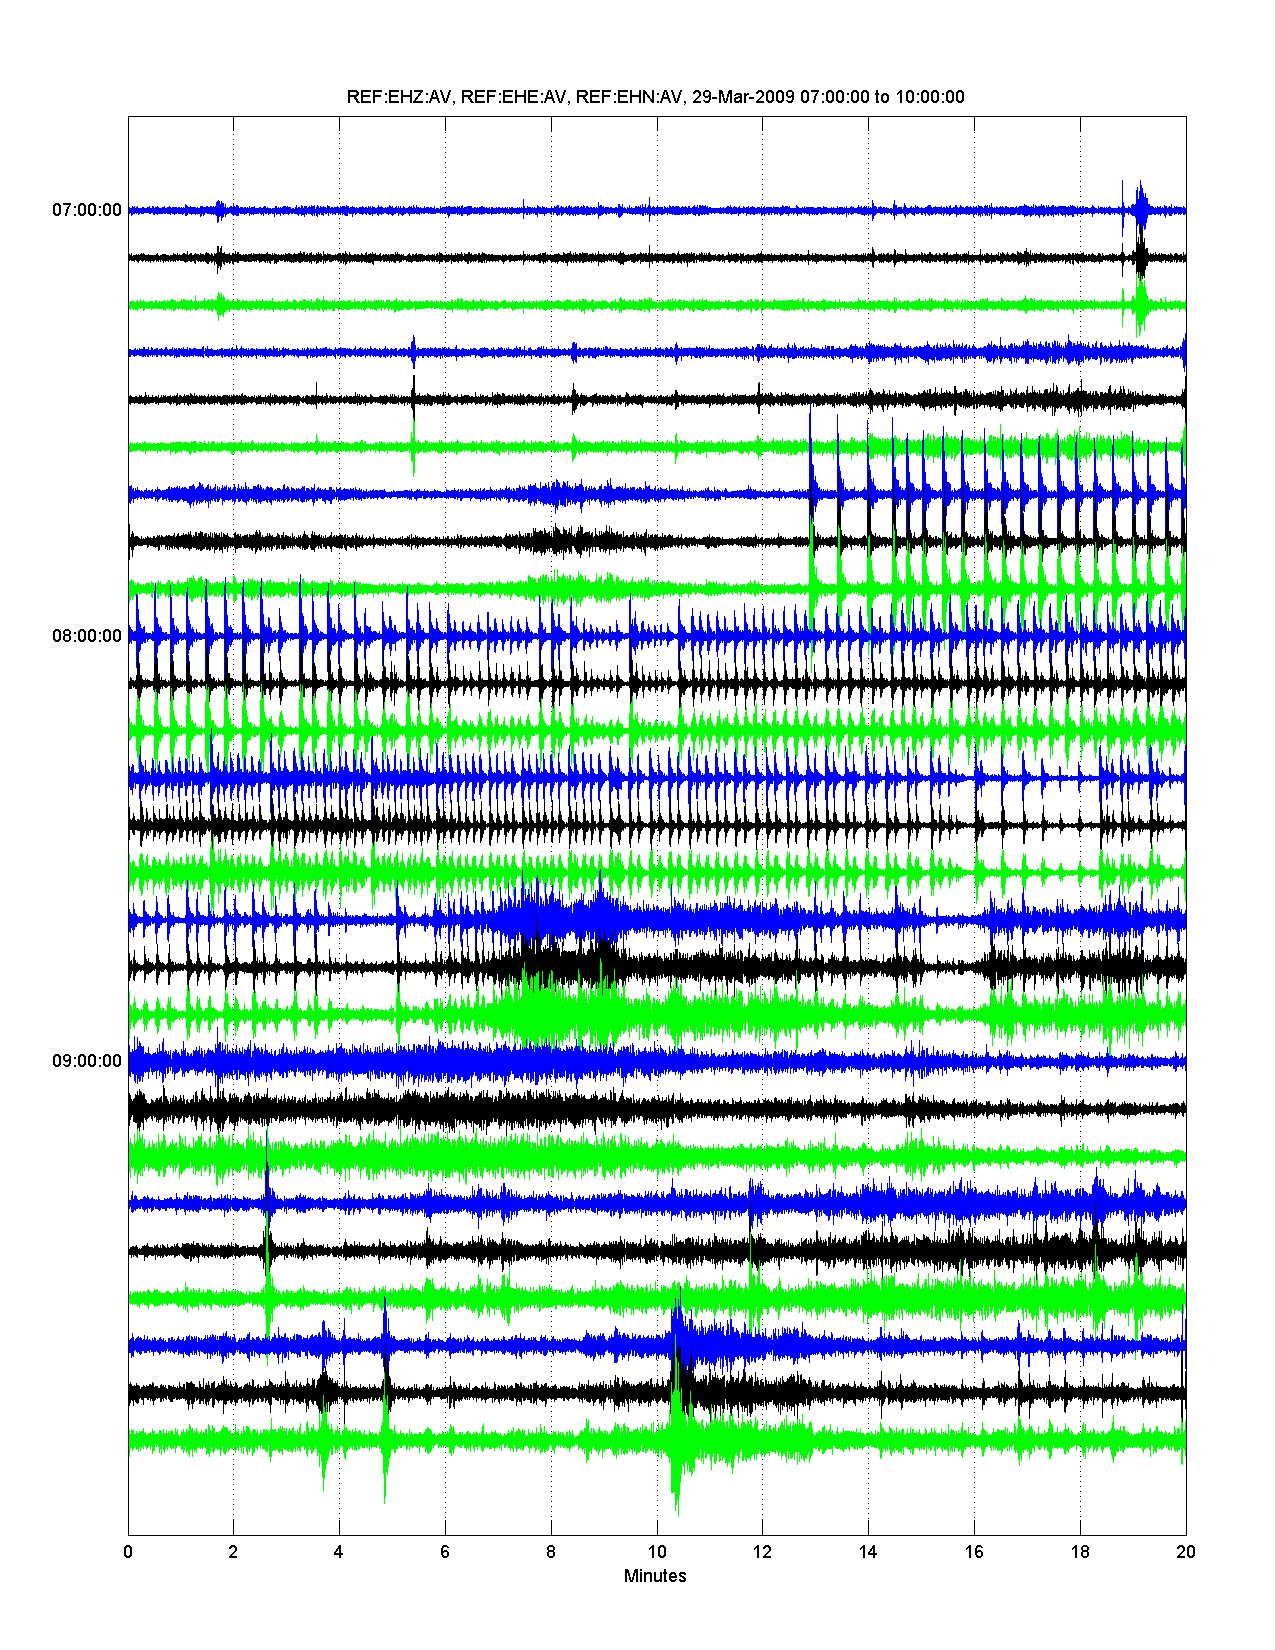
\includegraphics{hel_alternate_1.png}}} 
\caption{Default helicorder display for a 1x3 waveform} 
\label{hel_alternate_1}
\end{figure}
\clearpage

The multi-waveform display type can be changed from 'alternate' to 'group' or 'stack'. Setting display to 'group' will plot all trace data from the first element in \mcode{w} before starting the next. Figure~\ref{hel_group_1} displays the output from \mcode{build(helicorder(w,'mpl',20,'display','group'))}.

\begin{figure}[ht] 
\centerline{\scalebox{.6} {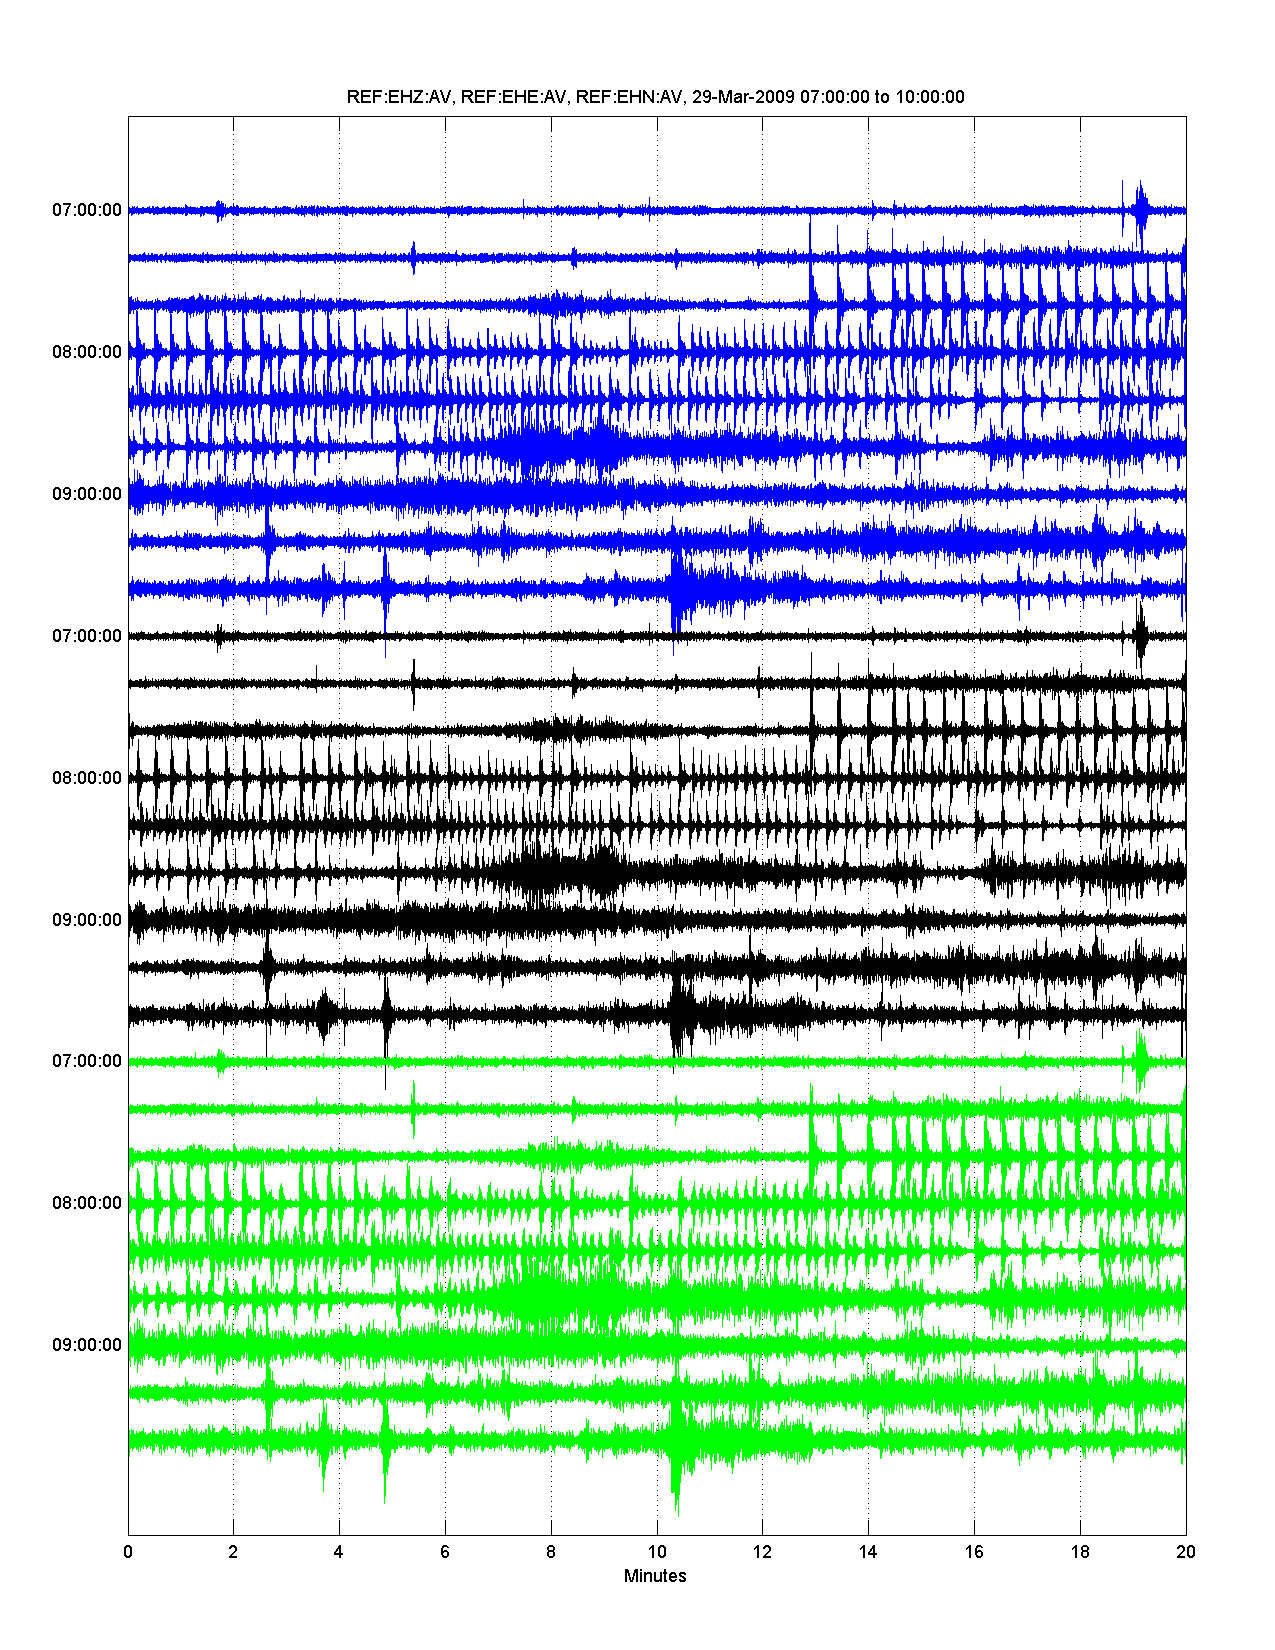
\includegraphics{hel_group_1.png}}} 
\caption{Multi-waveform 'group' display} 
\label{hel_group_1}
\end{figure}
\clearpage

The final multi-waveform display type is 'stack' which will plot waveforms one on top of the other. It should be noted that the default amplitude scaling of all waveforms is determined by the first waveform plotted in 'stack' mode, in this case \mcode{w(1)} is REF:EHZ. If separate amplitude scaling is desired for waveforms in w, it must be defined by the user. Figure~\ref{hel_stack_1} displays the output from \\ \mcode{build(helicorder(w,'display','stack'))}.

\begin{figure}[ht] 
\centerline{\scalebox{.6} {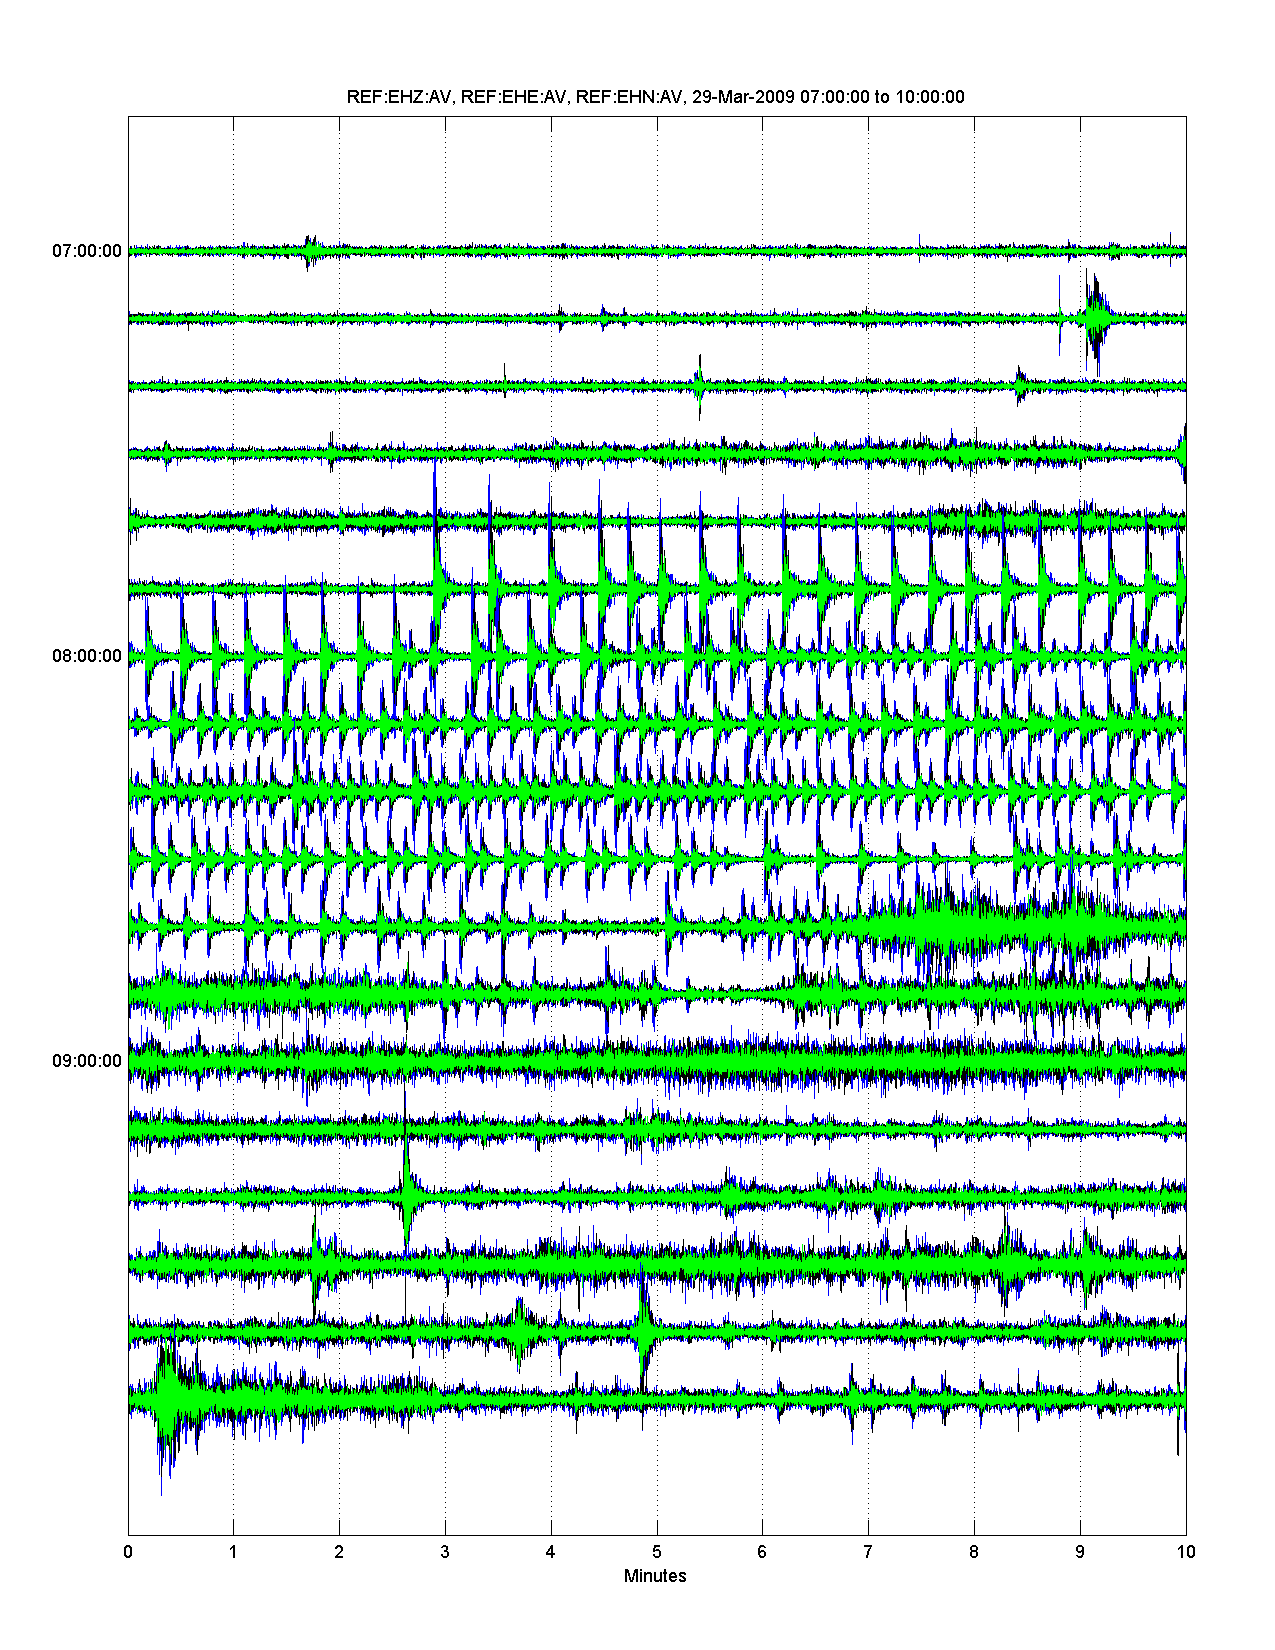
\includegraphics{hel_stack_1.png}}} 
\caption{Multi-waveform 'stack' display} 
\label{hel_stack_1}
\end{figure}

\clearpage

\subsection{Helicorder event overlay}

Helicorder can also be used to display discrete events from a waveform object. To do this, a set of event start/stop times (\mcode{sst1}) is required. Start/stop times can be manually picked, or can be the result of an auto-detection algorithm such as STA/LTA. 212 events are detected from the waveform data in Figure~\ref{hel_e_sst}. In our case, \mcode{sst1} is a 212x2 array of MatLAB times defining the begining and end of each event. Figure~\ref{hel_e_sst} displays the output from \mcode{build(helicorder(w,'mpl',15,'e_sst',sst1))} where \mcode{w} is broadband data from RDWB:BHZ from March 27, 2009 that has been band-pass filtered between 1 Hz and 10 Hz.

\begin{figure}[ht] 
\centerline{\scalebox{.6} {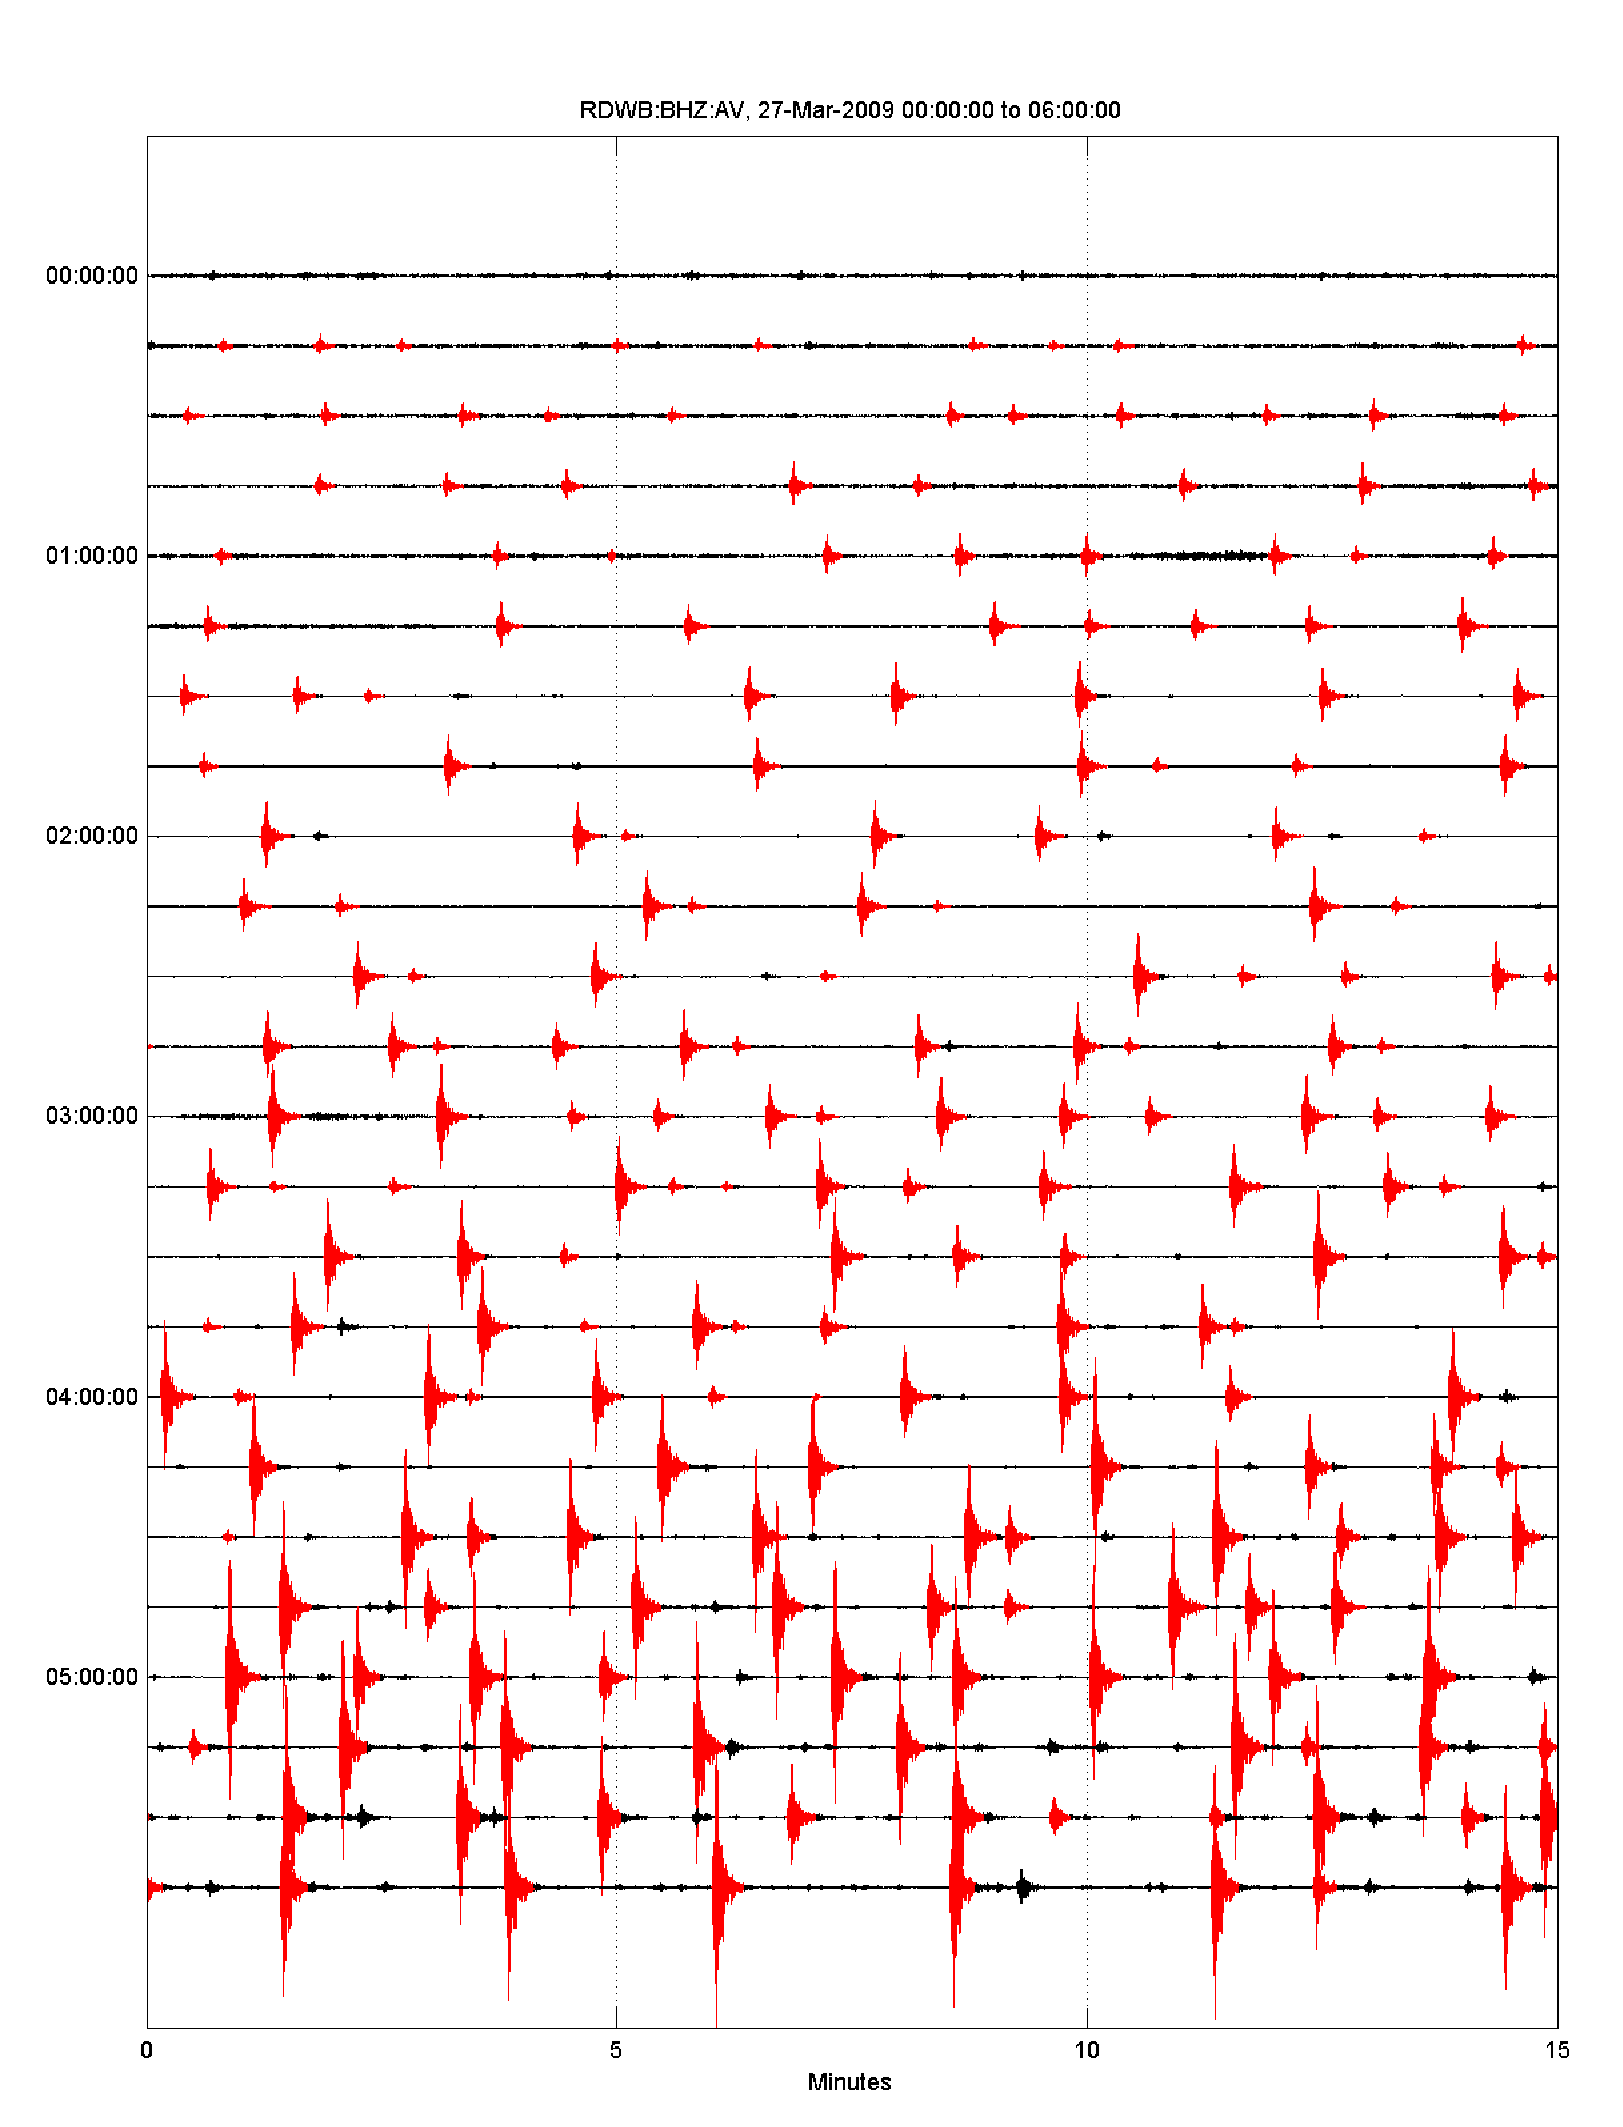
\includegraphics{hel_e_sst.png}}} 
\caption{Helicorder with event overlay} 
\label{hel_e_sst}
\end{figure}

\clearpage

\subsection{Helicorder VLP overlay example}

In the next example, \mcode{w} contains the unfiltered data from the previous event overlay example. Calling \mcode{build(helicorder(w,'mpl',15))} returns the following display:

\begin{figure}[ht] 
\centerline{\scalebox{.6} {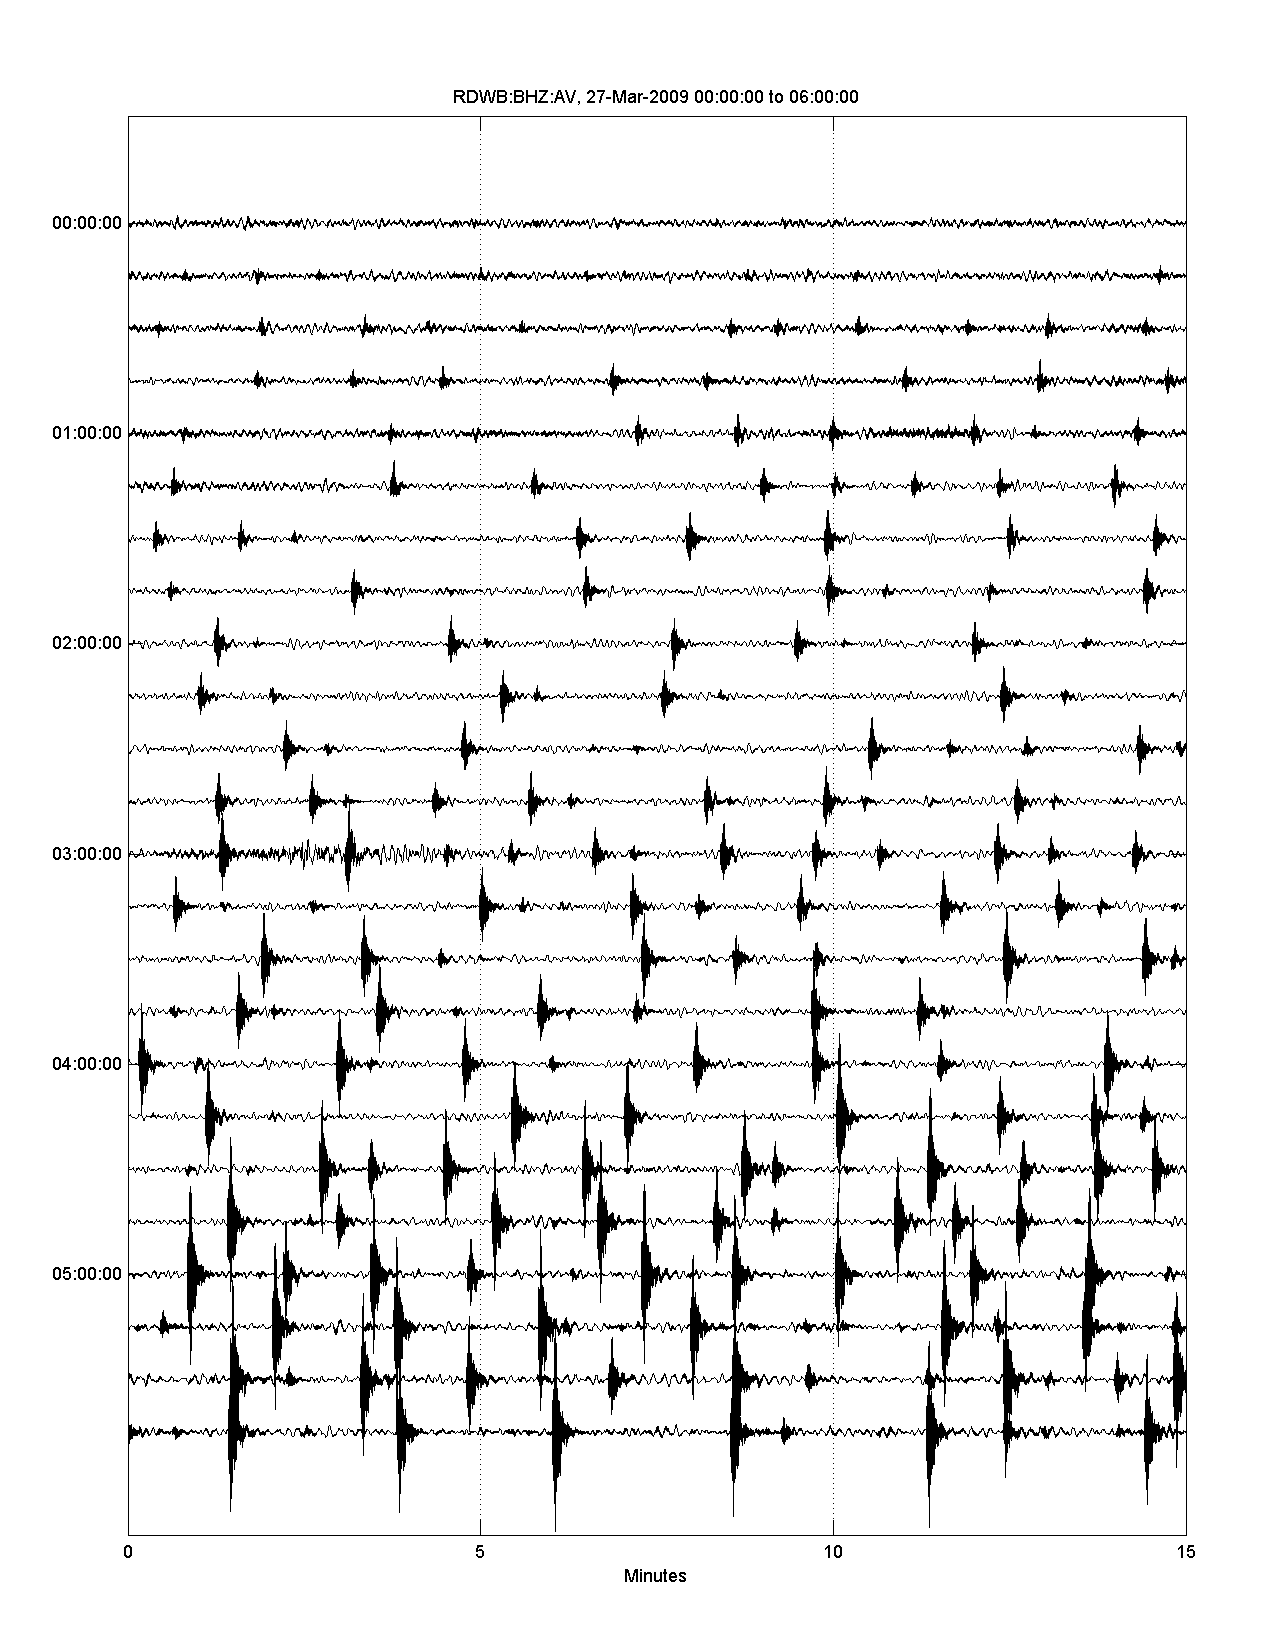
\includegraphics{hel_single_2.png}}} 
\caption{RDWB:BHZ helicorder} 
\label{hel_single_2}
\end{figure}
\clearpage

We suspect that there may be VLP energy in this data set, so we integrate \mcode{w} data to move from velocity to displacement. A second waveform \mcode{w_vlp} is created by filtering \mcode{w} over the VLP range (whatever you believe that might be). Next we combine \mcode{w} and \mcode{w_vlp} as follows: \mcode{w = [w w_vlp]}. This guarantees that VLP data is plotted on top of displacement data as seen in Figure~\ref{hel_stack_2}. We aren't satisfied with the default trace colors so we set them ourselves:  

\begin{lstlisting}
color = {[0 0 0],[1 0 0]}; % Normalized RGB value for black and red
build(helicorder(w,'mpl',15,'trace_color',color))
\end{lstlisting}


\begin{figure}[ht] 
\centerline{\scalebox{.6} {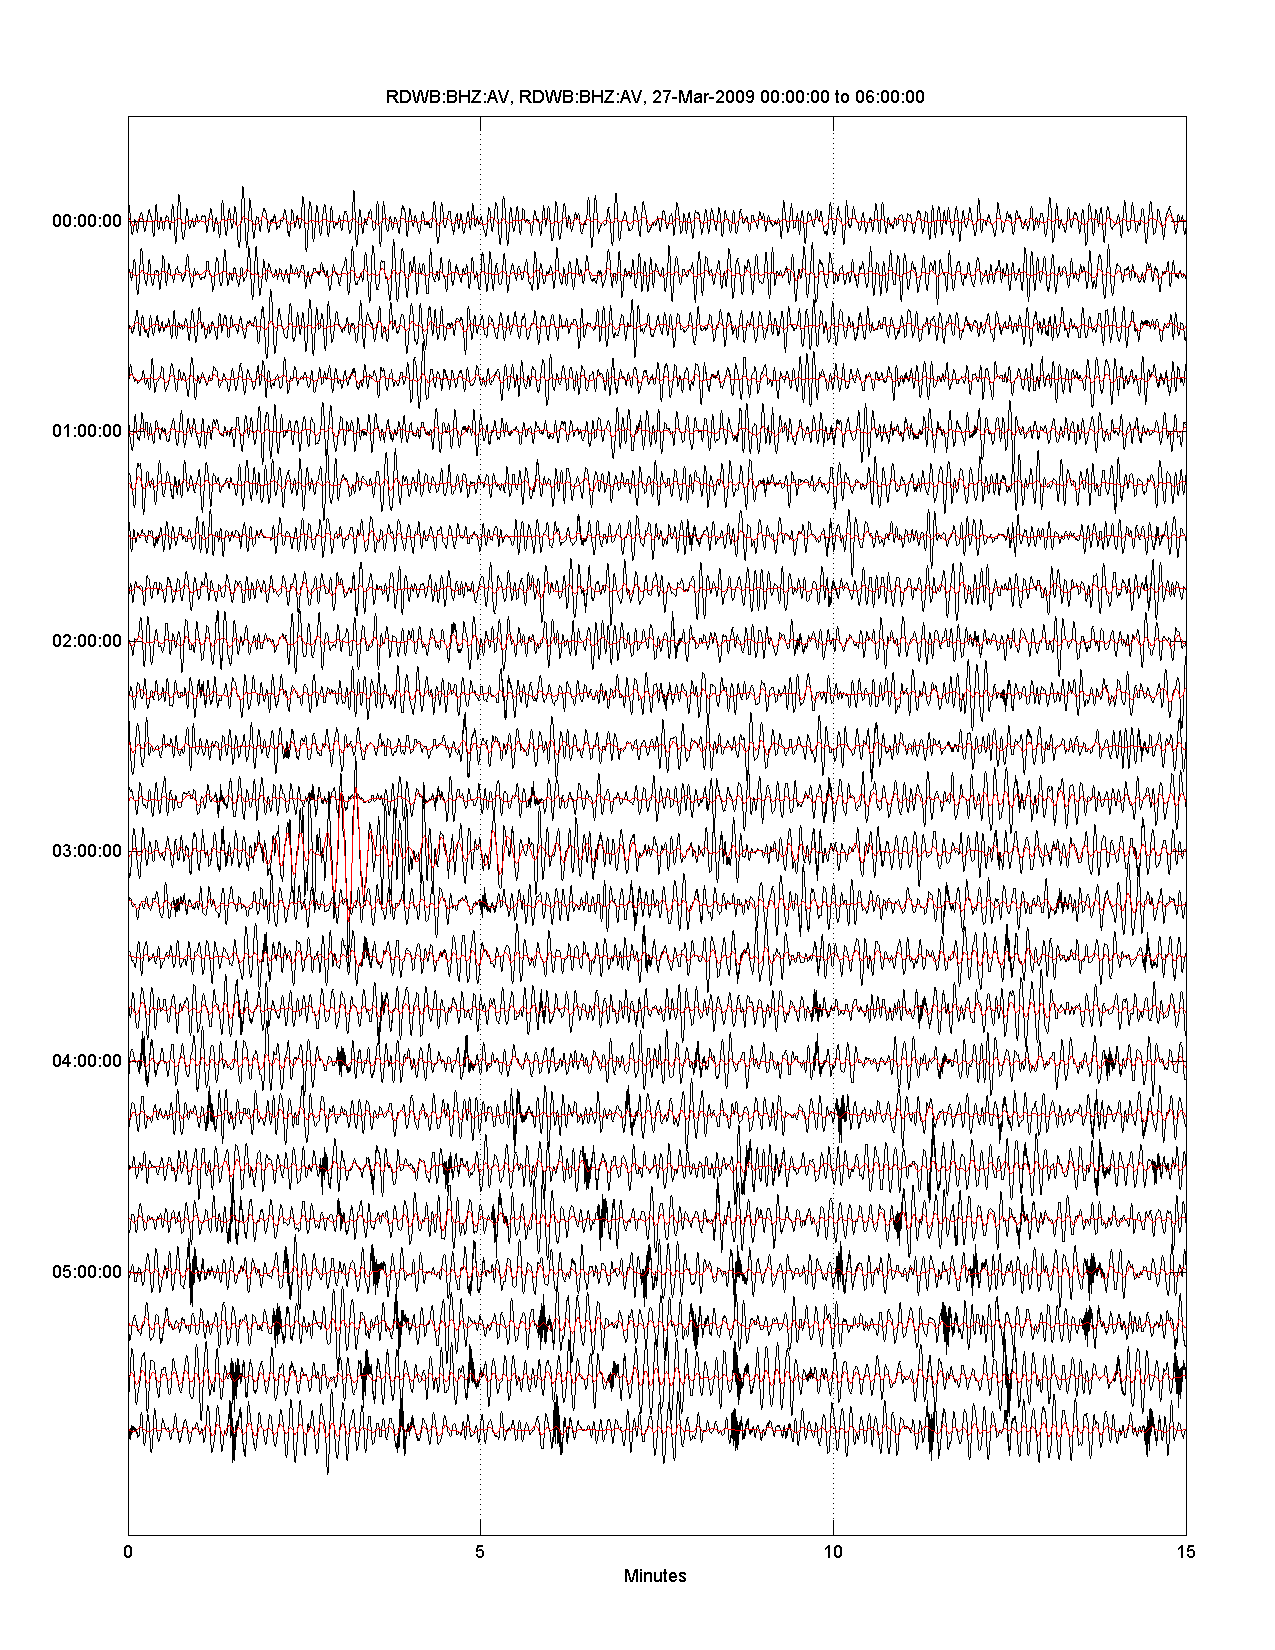
\includegraphics{hel_stack_2.png}}} 
\caption{Helicorder VLP overlay} 
\label{hel_stack_2}
\end{figure}

\clearpage

\subsection{Valid helicorder property name/value combinations}

\begin{itemize}
\item \mcode{e_sst} - Event Start/Stop Times \\
If wave contains only one wavefrom object, \mcode{e_sst} can be entered as an Nx2 array of matlab times. If there is more than one waveform in wave (M waveforms), \mcode{e_sst} must be a 1xM cell array, each cell containing Nx2 array of start/stop times. A single waveform can also have multiple sets of start/stop times as in a waveform with multiple event families. In this case \mcode{e_sst} should be entered as a 1xL cell array for a particular waveform (with L separate groups to be highlighted).
EXAMPLE: \mcode{h = helicorder(w,'e_sst',A)} where \mcode{w} is a 1x2 waveform object \\
\mcode{A} is a 1x2 cell array \\
\mcode{A(1,2)} is a 1x3 cell \\
\mcode{A(1,2)\{1\}} is a Nx2 numeric array \\
\mcode{A(1,2)\{2\}} is a Nx2 numeric array \\
\mcode{A(1,2)\{3\}} is a Nx2 numeric array \\
DEFAULT = [] (No events)

\item \mcode{mpl} - Minutes Per Line \\
single numeric value specifying number of minutes per helicorder line. (This applies to all waveforms in the helicorder)\\
DEFAULT = 10 

\item \mcode{ytick} - Y-Axis Ticks \\
single numeric value specifying number of minutes between y-axis tick marks and labels. 'ytick' depends on 'mpl', for example, if 'mpl' is 20, an attempt to set 'ytick' to 10 will be result in 'ytick' rounded to nearest multiple of 'mpl' (20 in this case). Note also that manually setting 'mpl' will result in an automatic adjustment of 'ytick'.\\
DEFAULT = 30

\item \mcode{trace_color} - Color Scheme of Trace Data\\
If \mcode{w} contains only one wavefrom object, \mcode{trace_color} can be entered as a 1x3 array of RGB values (between 0 and 1). For wave arguments longer than 1, \mcode{trace_color} should be entered as a 1xN cell array, each containing a 1x3 array of RGB values.

\item \mcode{event_color} - Color Scheme of Highlighted Event Data\\
Only use this property when \mcode{e_sst} property exists. \mcode{event_color} follows the same structure as \mcode{e_sst}. If wave contains only one waveform object, \mcode{event_color} can be entered as a 1x3 array of RGB values (between 0 and 1). For wave arguments longer than 1, \mcode{event_color} should be entered as a 1xN cell array, each containing a 1x3 array of RGB values. If multiple event sets exist for a single waveform, \mcode{event_color} must be specified accordingly.\\
EXAMPLE: \mcode{h = helicorder(w,'e_sst',A,'event_color',B)}\\
\mcode{A} is the same as the previous example\\
\mcode{B(1,1)} is a 1x3 RGB array\\
\mcode{A(1,2)} is a 1x3 cell\\
\mcode{A(1,2)\{1\}} is a 1x3 RGB array\\
\mcode{A(1,2)\{2\}} is a 1x3 RGB array\\
\mcode{A(1,2)\{3\}} is a 1x3 RGB array\\
DEFAULT = [] (No events)

\item \mcode{display} - Multi-Waveform Display Type\\
\mcode{'single'} - Used when there is only one waveform in wave. None of the multi-waveform display types can be set unless multiple waveforms are passed.\\
\mcode{'stack'} - Plots multiple waveforms over top of each other. (Multiple motivations could exist for wanting to display data in this way such as overlaying VLP energy).\\
\mcode{'alternate'} - Alternate through waveforms (grouped by time).\\
\mcode{'group'} - Plot all trace data in a waveform before starting the next (grouped by waveform source).\\
DEFAULT = 'single', 'alternate' (1 or multiple waveforms)

\end{itemize}

\subsection{Interacting with a helicorder figure}

The \mcode{build} fuction also provides a degree of interactivity with the helicorder figure. Clicking the cursor on any trace in the helicorder figure will call the function \mcode{traClick} from within \mcode{build}. The user can define what takes place after a helicorder trace line, or a highlighted event is clicked. By default, the GUI \mcode{sst_pick} is opened for the clicked waveform generating a minute-long waveform and spectral display.

Note: Helicorder interactivity is shut off by default as of this writing. If interested parties care to turn this on in the helicorder function build.m, they are welcome to.

\clearpage


\end{document}

